% ==================================================
% The CartPole Environment 
% Author: Lester James V. Miranda
% ==================================================

\documentclass[preview, convert={outfile=\jobname-out.png,density=300}]{standalone}

\usepackage{tikz}
\usepackage{color}
\usepackage{subfig}
\usepackage{ifthen}
\usepackage{graphicx}
\usepackage{fontawesome}

\renewcommand\familydefault{\sfdefault}

\usetikzlibrary{
    matrix,
    shapes,
    fit,
    arrows,
    positioning,
    calc,
    backgrounds,
    shadows.blur,
    shapes.geometric,
}

\begin{document}
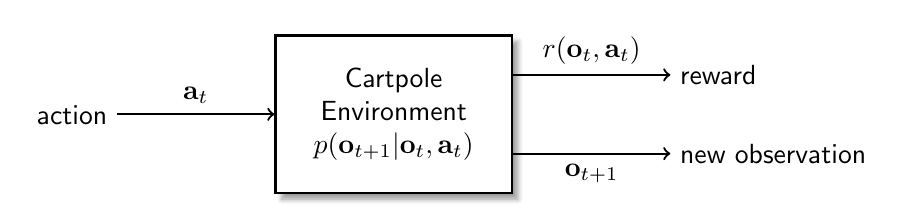
\begin{tikzpicture}[
    state/.style={draw, thick, align=center, minimum width=3cm, minimum height=2cm, fill=white, text=black, blur shadow={shadow blur steps=5}},
    ]

\node[state] at (0,0) (cartpole)
    {Cartpole\\Environment\\$p(\mathbf{o}_{t+1} \vert
    \mathbf{o}_{t}, \mathbf{a}_{t})$};

\draw[->, thick] ([yshift=0.5cm]cartpole.east) -- ++(2,0) 
    node[midway, above] (out1) {$r(\mathbf{o}_{t}, \mathbf{a}_{t})$};

\draw[->, thick] ([yshift=-0.5cm]cartpole.east) -- ++(2,0) 
    node[midway, below] (out2) {$\mathbf{o}_{t+1}$};

\node[anchor=west] at ([xshift=1cm]out1.south) {reward};

\node[anchor=west] at ([xshift=1cm]out2.north) {new observation};

\draw[<-, thick] (cartpole.west) -- ++(-2,0) 
    node[midway, above] (in1) {$ \mathbf{a}_{t}$};

\node[anchor=east] at ([xshift=-1cm,yshift=-0.25cm]in1) {action};

\end{tikzpicture}
\end{document}
